%!TEX root = ../Thesis.tex
\chapter{Experimental results}
\label{sec:results}

%--------------------------------------------------------------------------------
\clearpage
\section{Initial investigation: WAFFLE experiment}
\label{sec:waffle}

Placeholder

%--------------------------------------------------------------------------------
\clearpage
\section{Addendum: Key results and lessons learned}
\label{sec:waffle_addendum}

Placeholder

%--------------------------------------------------------------------------------
\clearpage
\section{Introduction to second study: \newline 
{\O}sterild Balconies experiment}
\label{sec:balcony_intro}

\begin{comment}
Necessary to measure at zero elevation angle
Avoid influence from terrain and vegetation
Similar to offshore conditions
Scope of NEWA project fit well into this thesis
\end{comment}

%--------------------------------------------------------------------------------
\clearpage
\section{Minute-Scale Wind Speed Forecasting Using Scanning Lidar Inflow Measurements}
\label{sec:balcony_paper}

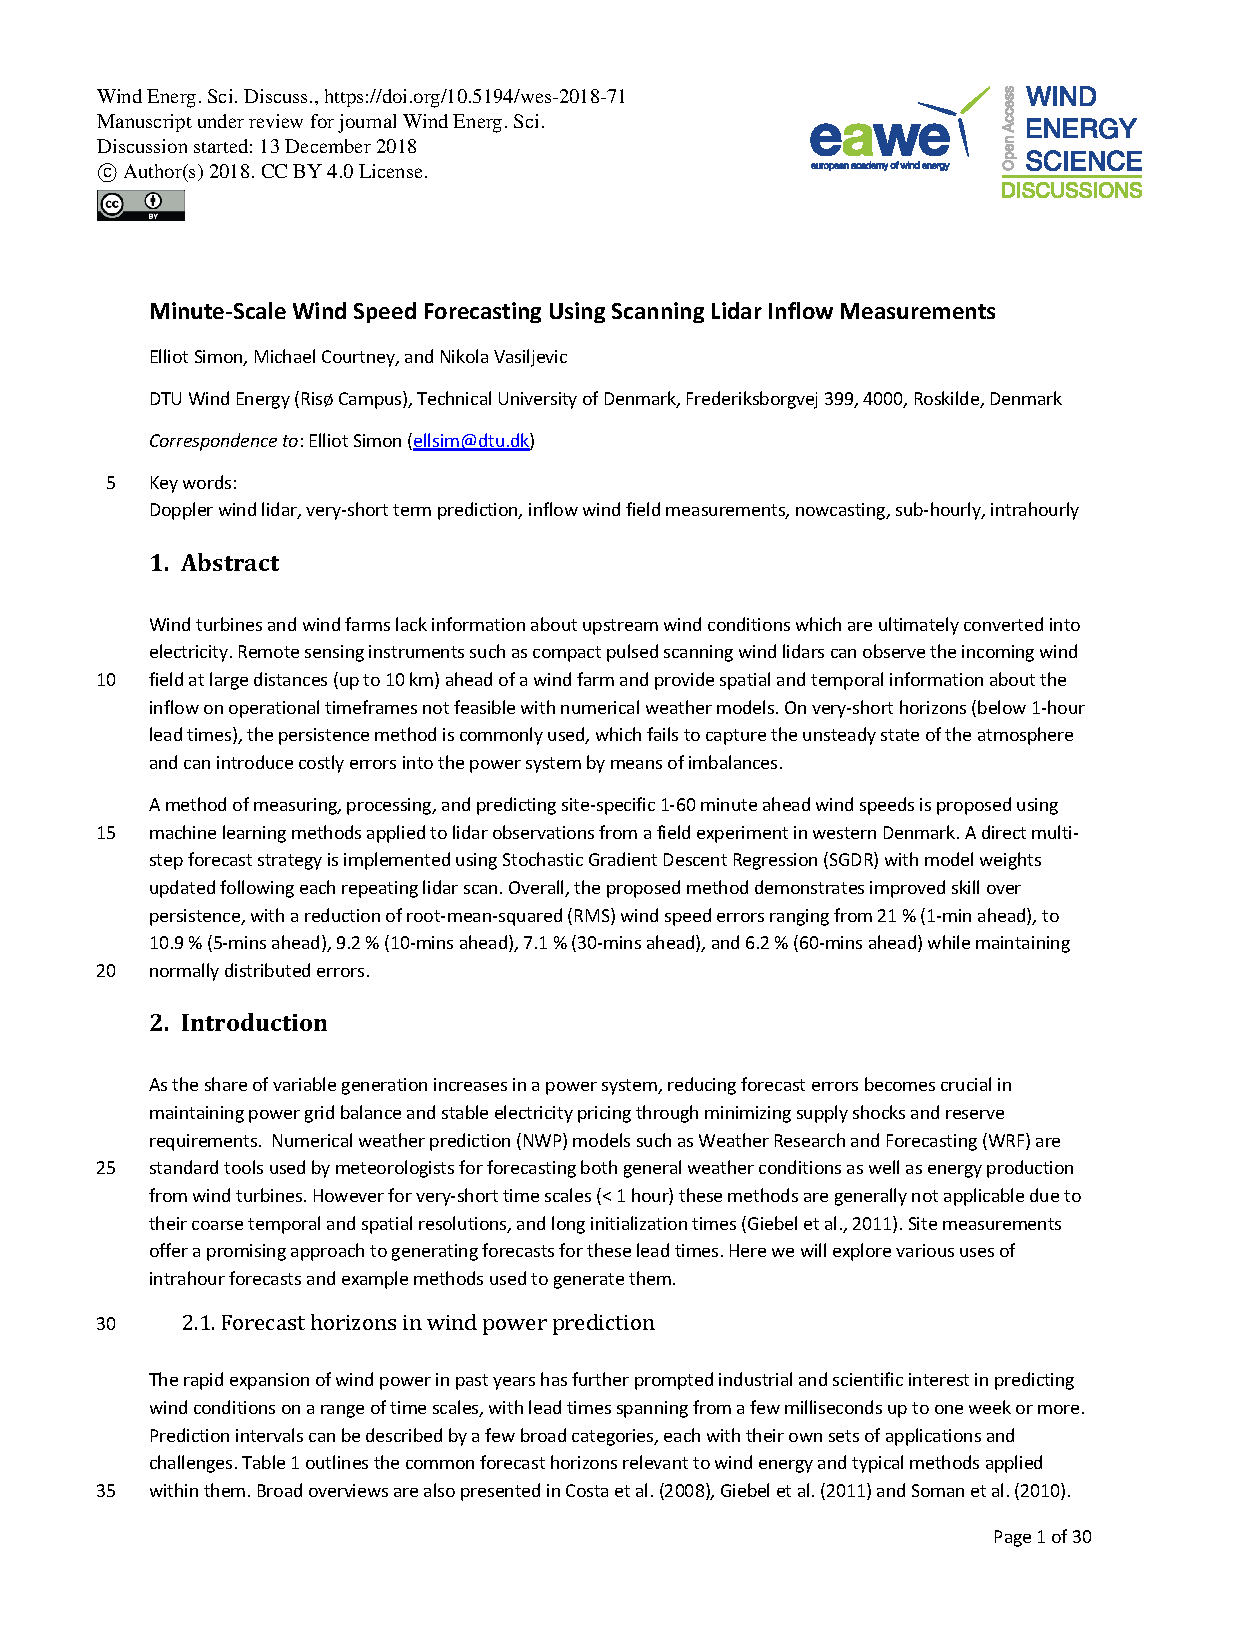
\includepdf[pages=-]{papers/Balcony_paper_WESD.pdf}

%--------------------------------------------------------------------------------
\clearpage
\section{Addendum 1: Weather front event}
\label{sec:balcony_addendum1}

This section expands upon an oral presentation titled "Lidars Lifted: The {\O}sterild Balconies Experiment" given at the 97th American Meteorological Society (AMS) conference in Seattle (\cite{simon_lidars_lifted_2017}).

During the first phase of the Balconies experiment while the scanning lidars were deployed at 50 m above ground level (AGL),
a weather event was encountered with a potentially high impact for an operational wind turbine or wind farm.

At approximately 7PM on the 6th of June 2016, the arrival of a cold front drastically changed the wind regime at the test site. Although it did not cause a significant wind speed ramp, the wind directions of the two air masses were diametrically opposed. The result was a near instant 180 degree shift in wind direction (from 130 to 310 degrees) as the frontal advection displaced the formerly presiding conditions. 

This example of sudden and extreme veer has undesired and potentially damaging effects for a wind turbine. From an energy production perspective by requiring significant time and control adjustments to adapt to the new conditions, and from a loads perspective by introducing a sudden and extreme loading of the rotor and tower structure which is outside of normal operating conditions.

Figure \ref{fig:balcony-front-mast} presents a meteorological look into the event using measurements from the northern aircraft warning tower at {\O}sterild.

\begin{figure}[htbp]
    \centering
        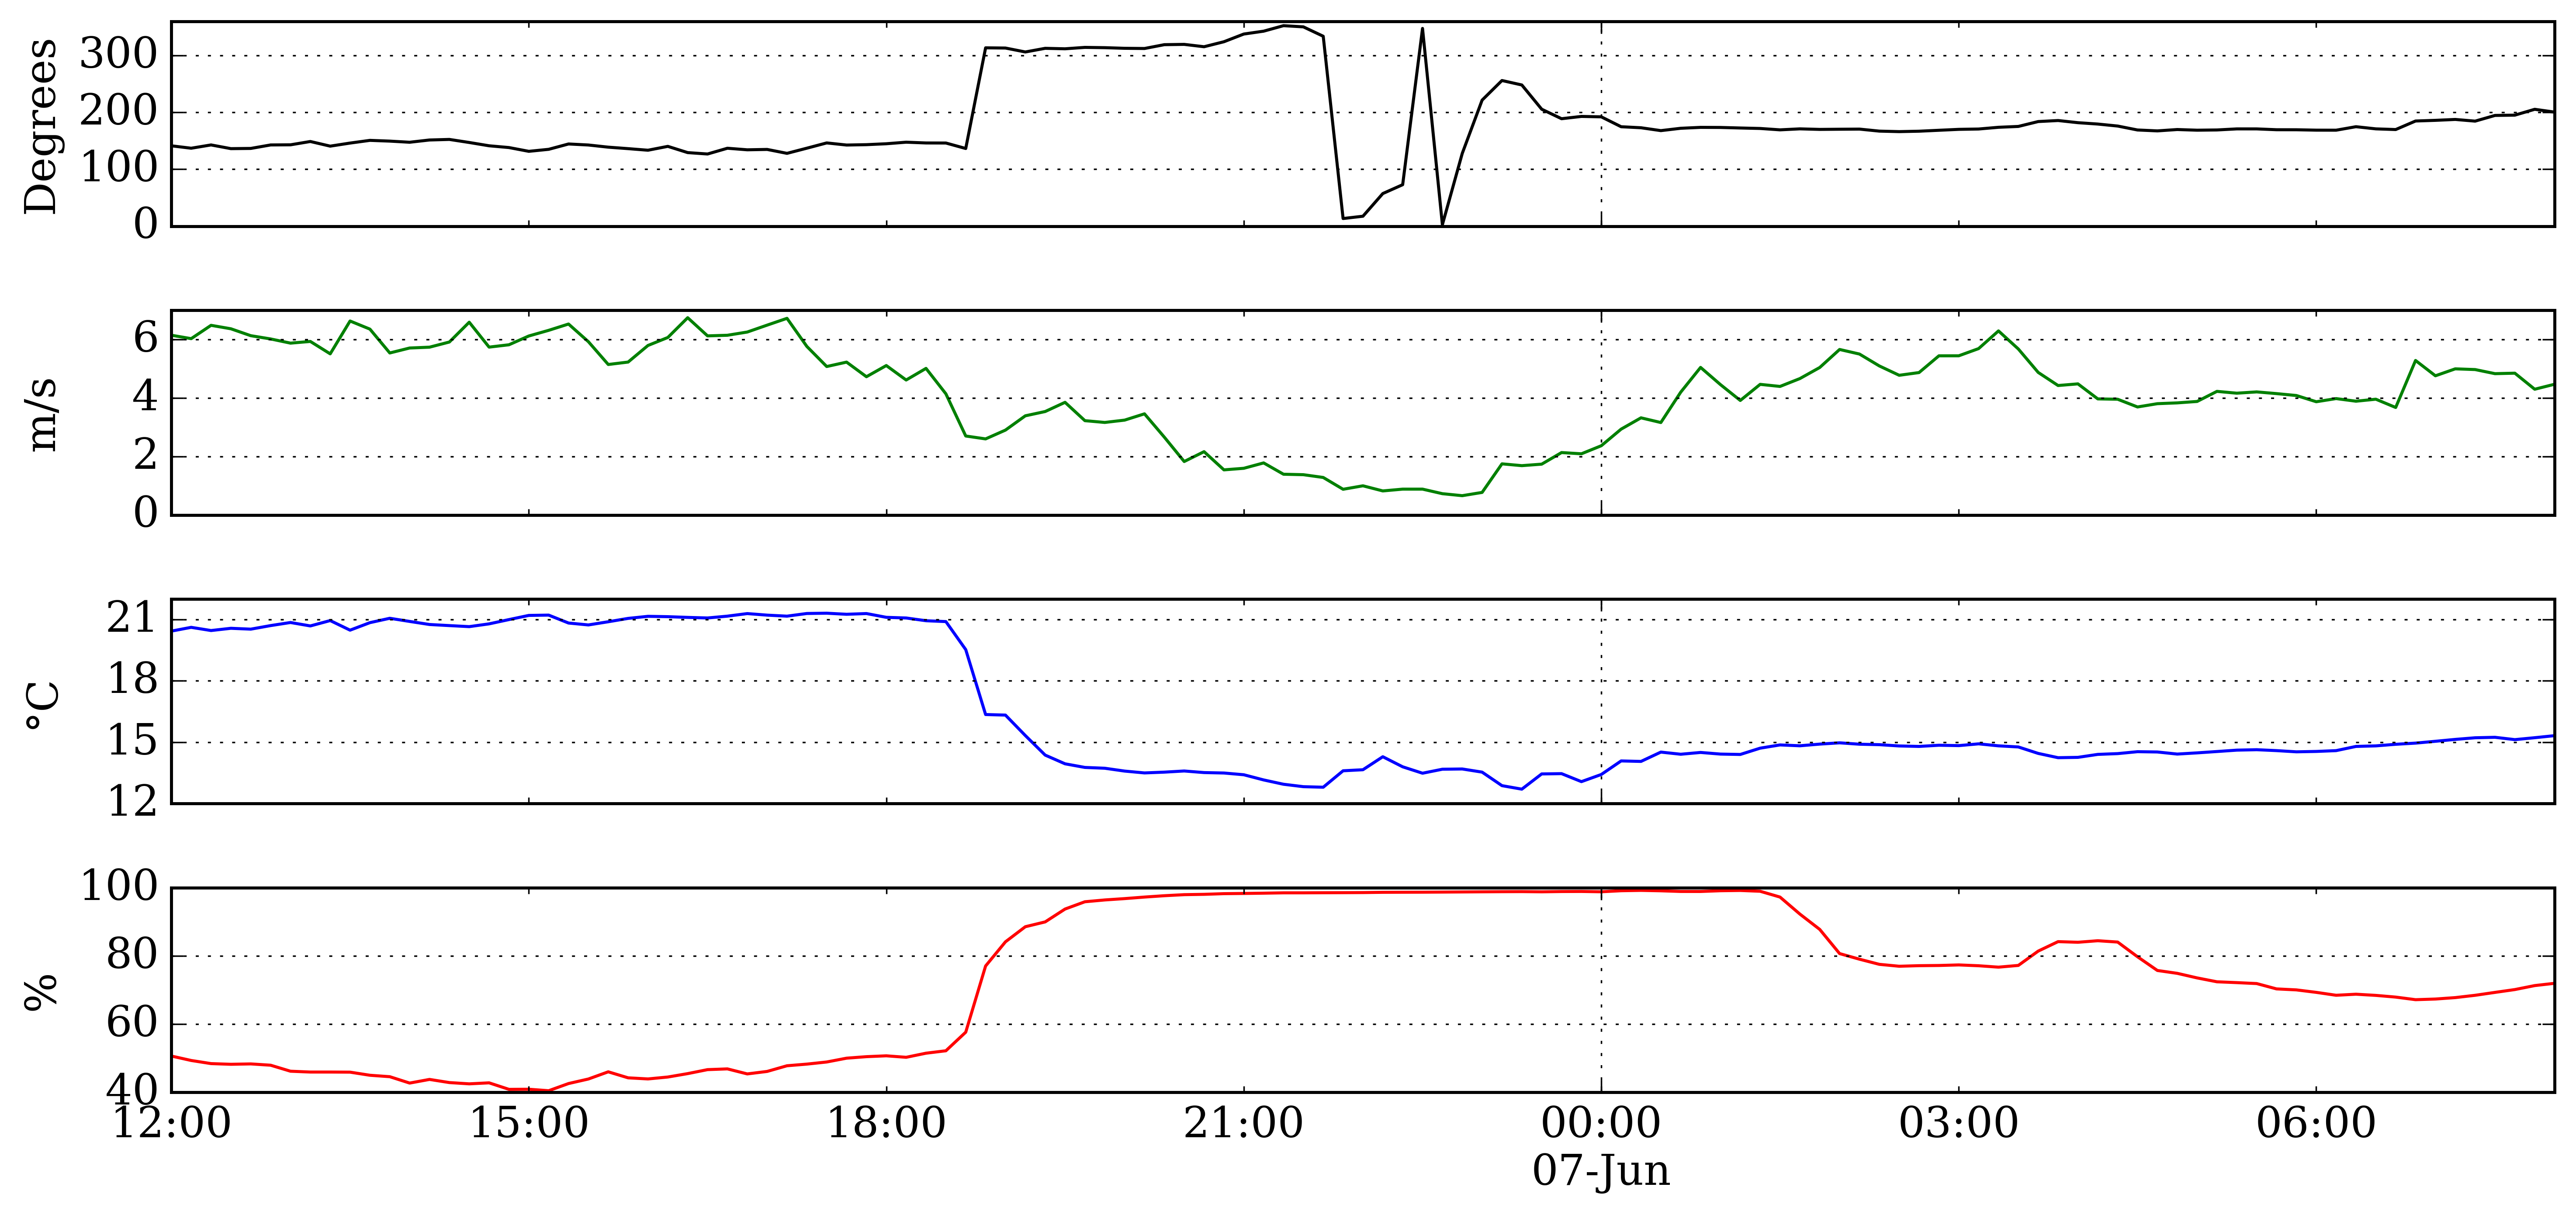
\includegraphics[width=1.0\textwidth]{graphics/results/balcony-addendum/balcony-front-mast.png}
    \caption{Mast measurements during a passing cold front at {\O}sterild test center on June 6-7, 2016.
    Top panel: Wind direction at 40 m AGL. Second panel: Wind speed at 40 m AGL. Third panel: Temperature at 37 m AGL. Bottom panel: Relative humidity at 7 m AGL}
    \label{fig:balcony-front-mast}
\end{figure}

<add lidar obs here>


\begin{figure}[htbp]
    \centering
        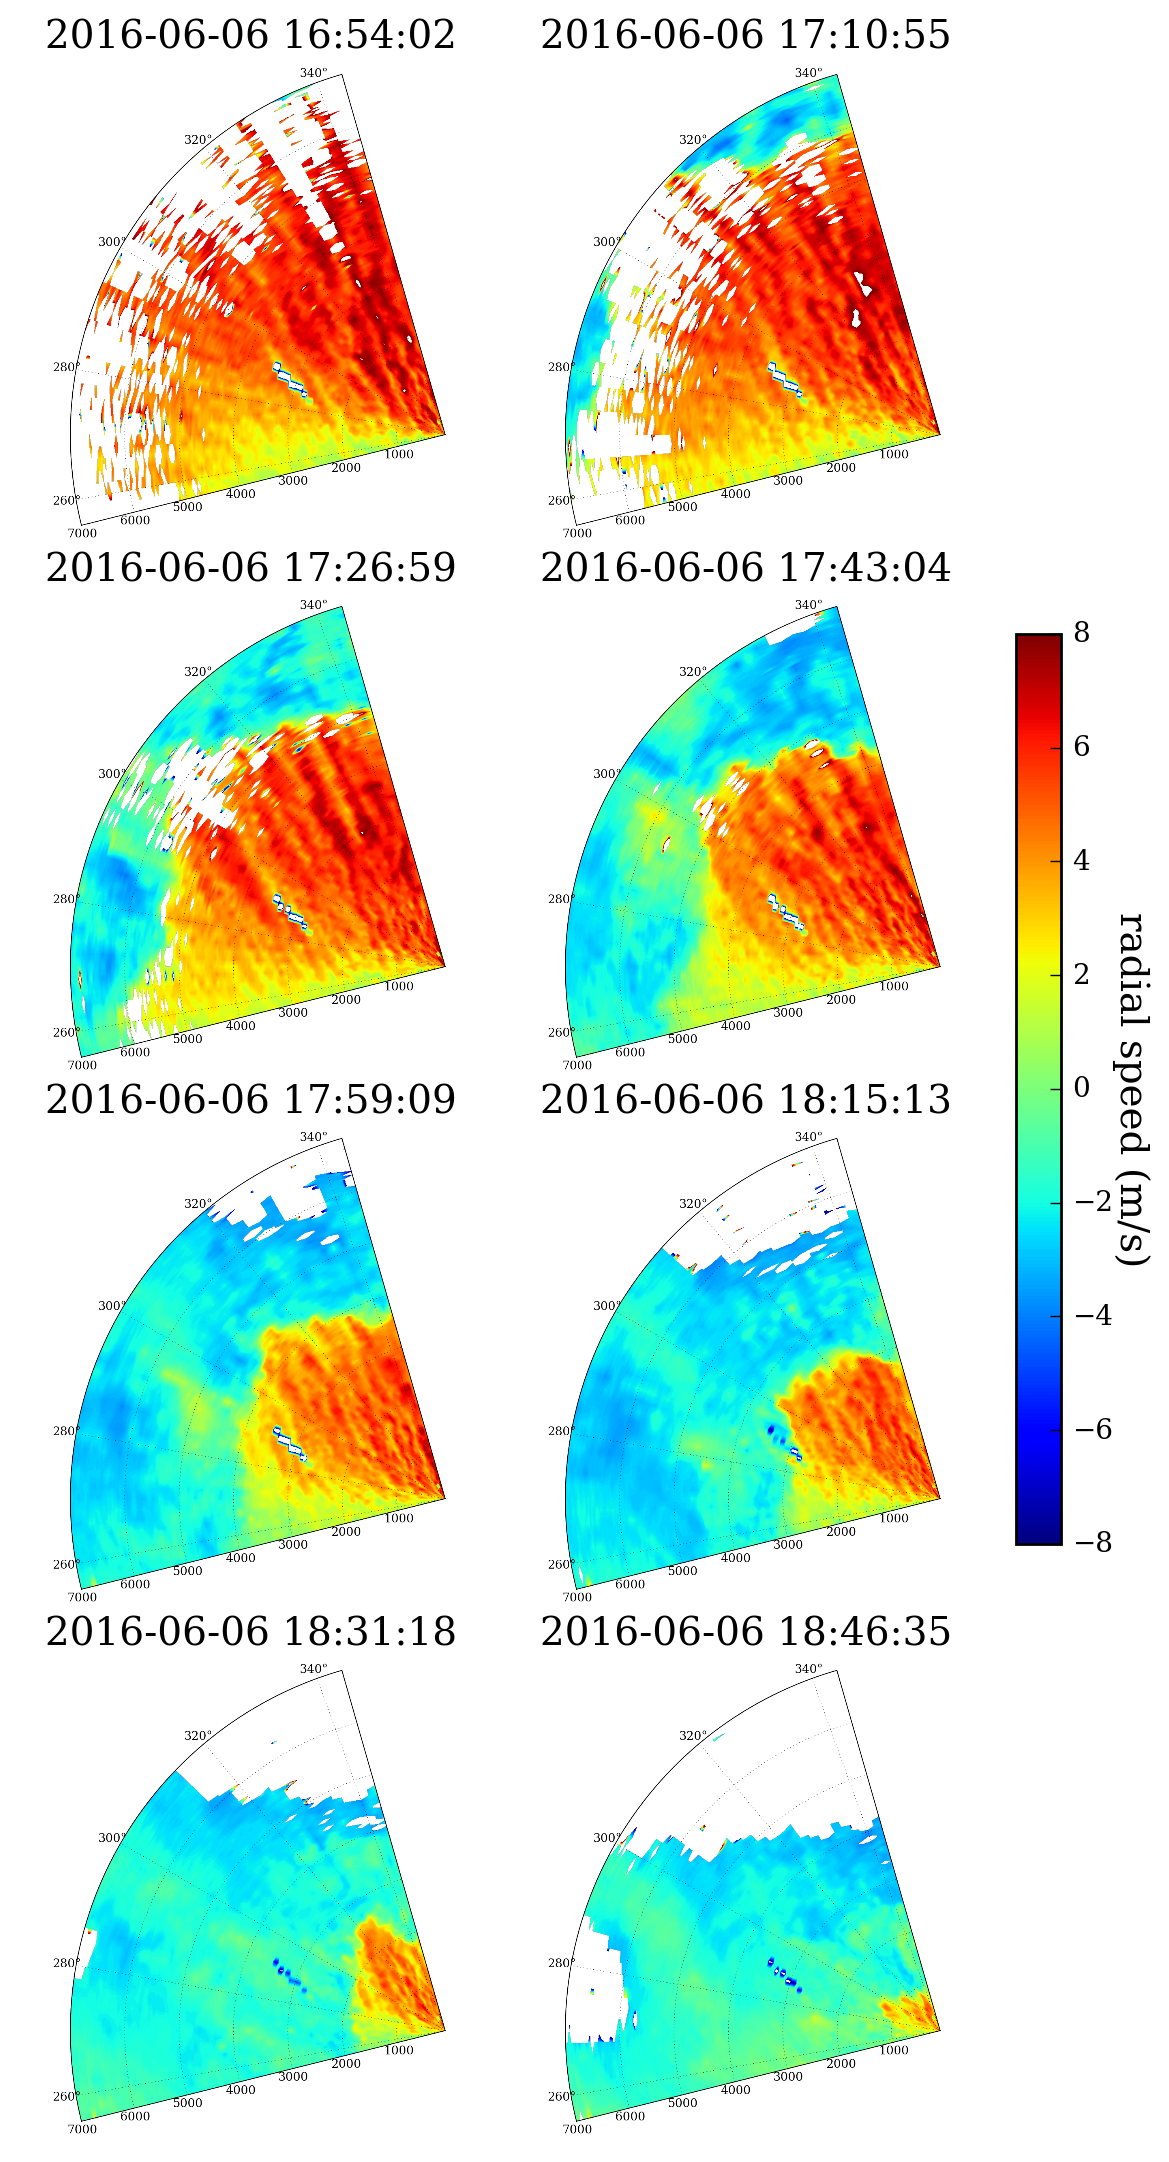
\includegraphics[width=1.0\textwidth, height=1.0\textheight, keepaspectratio]{graphics/results/balcony-addendum/lidar_front_ppis_8up.png}
    \caption{Lidar observations}
    \label{fig:lidar_front_ppis_8up}
\end{figure}

This event is an example of a very difficult to forecast phenomenon. Statistical methods including persistence and autoregressive (AR) models will fail spectacularly as there is no connection between the recent past and what lies ahead. While physical approaches including numerical weather prediction (NWP) models are in many cases able to predict the existence of a passing weather front, correctly predicting the timing (phase error) is notoriously difficult.

To further examine the usefulness of the upwind lidar system in capturing the event, predictions from an NWP model were compared with the local site measurements. 
Weather Research and Forecasting (WRF) version 3.5.1 model outputs at 2 km spacial resolution and 1 hour temporal resolution were obtained from Andrea Hahmann at DTU Wind Energy. The domain is shown in Figure \ref{fig:wrf_grid_annotated} along with the grid cell nearest to the met-mast. The distance from the met-mast position to the nearest grid cell is 1.16 km.

\begin{figure}[htbp]
    \centering
        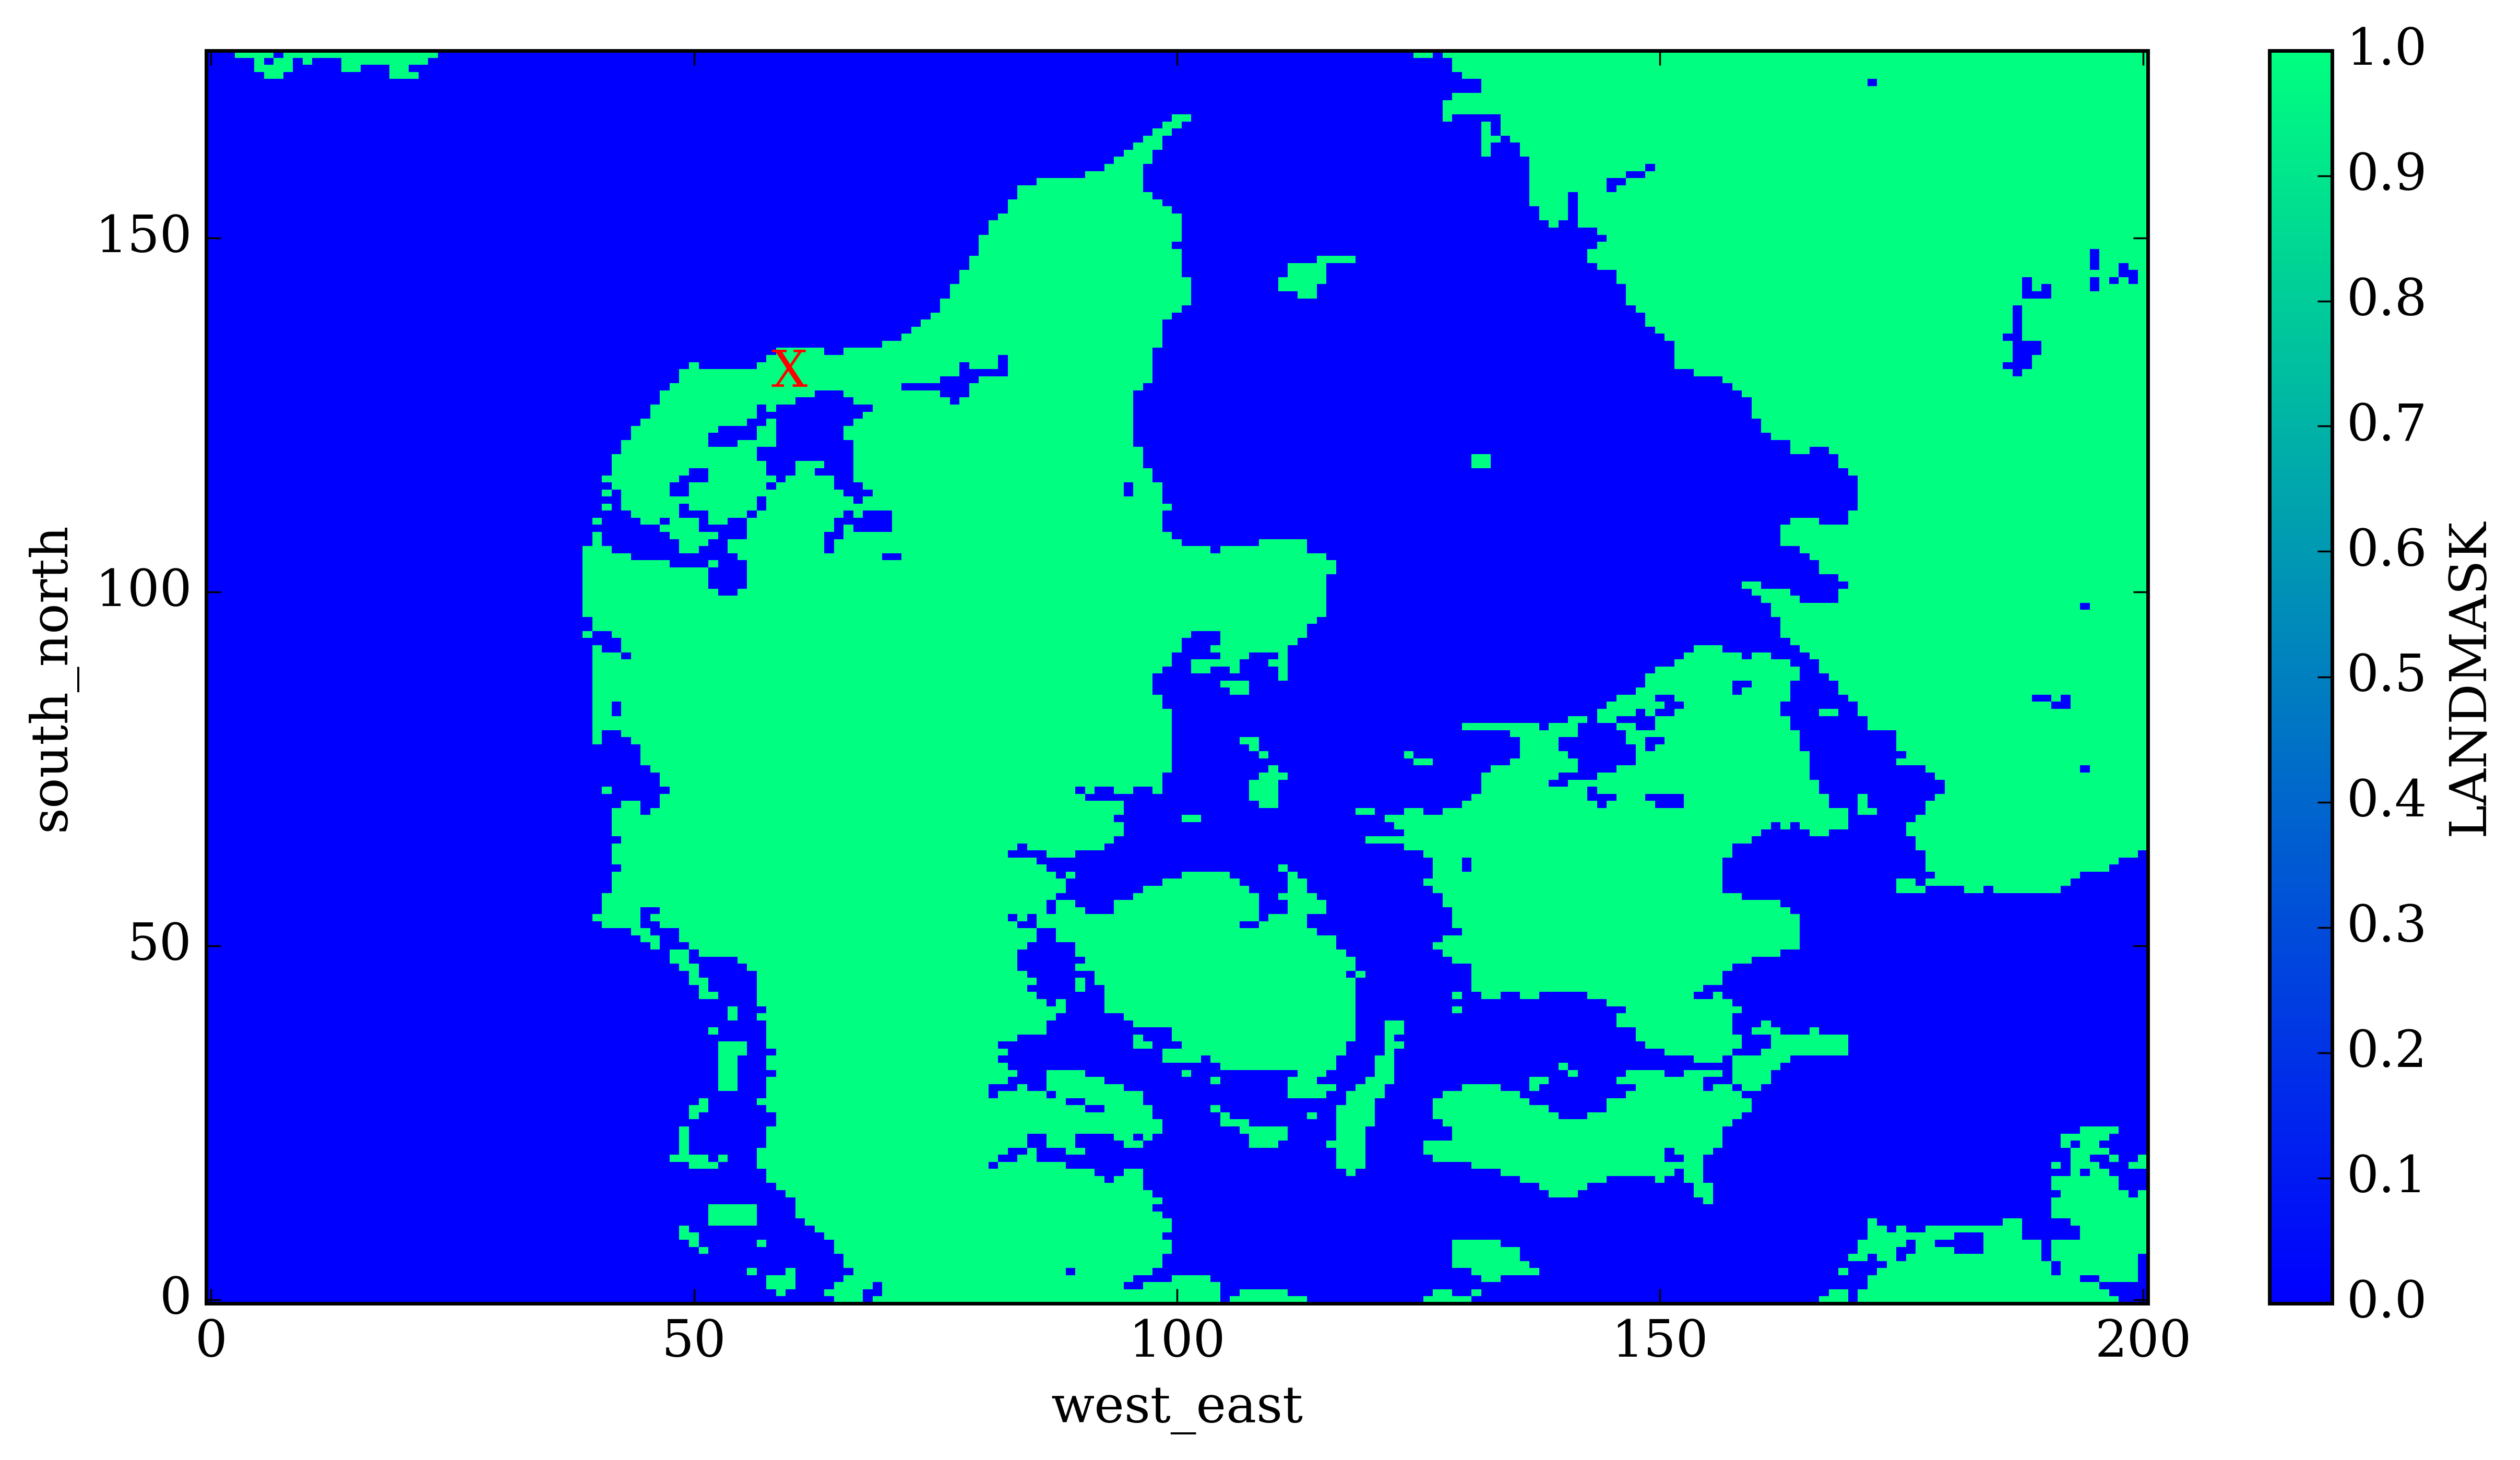
\includegraphics[width=0.75\textwidth]{graphics/results/balcony-addendum/wrf_grid_annotated.png}
    \caption{Domain for WRF simulation, with a red X denoting the grid cell nearest to the met-mast}
    \label{fig:wrf_grid_annotated}
\end{figure}

Four runs: two initialized on June 5th at 0Z (midnight UTC) and 12Z (noon UTC), and two initialized on June 6th (0Z and 12Z) were used to make comparisons between wind speed and direction predictions and the actual site measurements. Model predictions have all been converted to the CET time zone for synchronization with the met-mast data.

<add in plot of model comparisons>

<add in evaluation and concluding remarks>














captured and tracked propogation of cold front






%--------------------------------------------------------------------------------
\clearpage
\section{Addendum 2: Key results and lessons learned}
\label{sec:balcony_addendum2}

Placeholder


%--------------------------------------------------------------------------------
\clearpage
\section{Introduction to third study: LASCAR experiment}
\label{sec:lascar_intro}

Placeholder


%--------------------------------------------------------------------------------
\clearpage
\section{Minute-Scale Wind Vector Forecasting Using Scanning Lidar Inputs to a Convolutional LSTM Neural Network}
\label{sec:lascar_paper}

Placeholder for LASCAR paper
%\includepdf[pages=-]{papers/LASCAR_paper.pdf}

%--------------------------------------------------------------------------------
\clearpage
\section{Addendum: Key results and lessons learned}
\label{sec:lascar_addendum}

Placeholder